\noindent In this doctoral thesis I have presented three searches for new heavy ($>1 TeV$) resonances decaying to two vector bosons in the all-hadronic final state, using datasets collected by the CMS experiment corresponding to an integrated luminosity of 2.5(2015), 35.9(2016) and 77.8(2016+2017) \fbinv. Due to the high energy ("boost") of the vector bosons, their decay products are so collimated that they get merged into one single jet, leading to a dijet final state topology.
Dedicated jet grooming and jet substructure techniques are therefore explored in order to discriminate vector bosons from the overwhelming QCD multijet background.\newline 
Each of the analyses presented has provided original contributions to the field: The first search was the first of its kind to ever be performed at $\sqrt{\rm{s}}=13 \TeV$, following an observed excess of 3.4 (1.3) $\sigma$ by ATLAS (CMS) in the 8 \TeV dataset, and the first time CMS demonstrated the efficiency of using jet grooming techniques at trigger level. It, at the time, set the most stringent limits to date for the signal scenarios under consideration.\newline
The second search introduces a novel pileup resistant and perturbative safe vector boson tagging algorithm based on PUPPI softdrop jet mass, ensuring a high and stable signal efficiency up to pileup of at least 50 interactions per event. The optimization, validation and full commissioning of the tagger was performed in the context of this search. Dedicated jet mass corrections in order to account for an observed \PT and $\eta$ dependence in PUPPI softdrop jet mass, due to the nature of the softdrop algorithm, were also developed. The PUPPI softdrop based tagger, together with the jet mass corrections, became, and still is, the recommended algorithm for W-tagging in CMS. \newline
The final analysis introduces a band new way of doing diboson resonance searches through a tree dimensional fit of the dijet invariant mass and the softdrop mass of the two jets. By optimization of the W-tagging algorithm used in this search and the nature of the search method, we have, for the first time, been able to extract the jet mass scale and resolution for a merged  $\PW(\bar{\rm{q}}\rm{q})$ and $\PZ(\bar{\rm{q}}\rm{q})$ peak from the V+jets Standard Model process. The method itself leads to a 20-30 \% higher sensitivity than the default search method. 
\newline
\newline
The benefit of using a three-dimensional fit based on dijet invariant mass and the softdrop jet masses of the two jets, is that one can look for resonances peaking anywhere in the jet mass and dijet invariant mass spectrum.

\begin{figure}[h!]
\centering
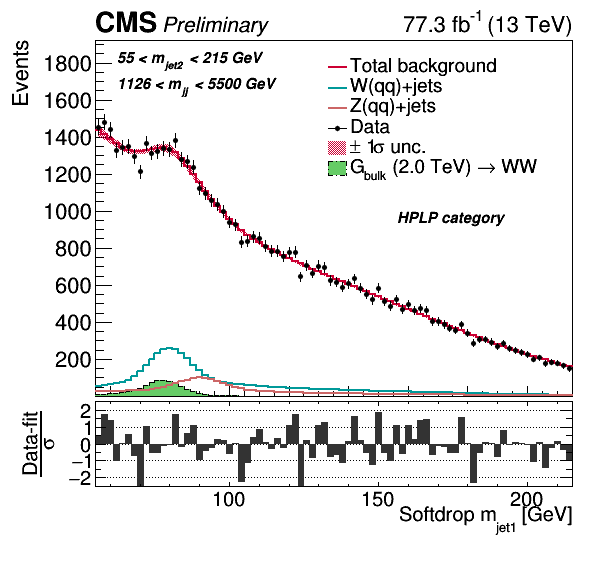
\includegraphics{figures/analysis/search3/AN-17-303/postfitchecks/postfit_HPLP_unblind/PostFitComboHPLP_X-Proj__y___0_-1_z___0_-1.pdf}

\label{fig:summary}
\end{figure}